\section*{Figures}

\listoffigures

\clearpage

\begin{figure}[tbhp!] \centering
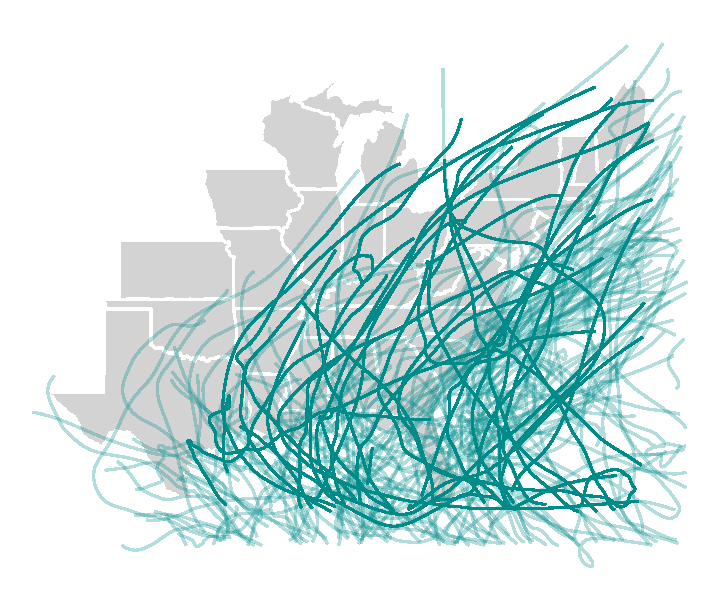
\includegraphics[width=0.7\linewidth]{hurrtracks}
\caption{States and storms considered in this study. All counties in the states
	shown in this map were investigated. The lines show the paths of the
	study storms, which included all tracked storms in 1988\,--\,2015 that
	are recorded in \ac{HURDAT2}~\parencite{landsea2013} and that came
	within 250~\si{\kilo\metre} of at least one \ac{US} county. Thicker
	lines show the tracks of storms whose names have been retired,
	indicating that the storm was particularly severe or had notable
	impacts~\parencite{retirednames}.  }
\label{fig:hurrtracks}
\end{figure}

\clearpage

\begin{figure}[tbhp!] \centering
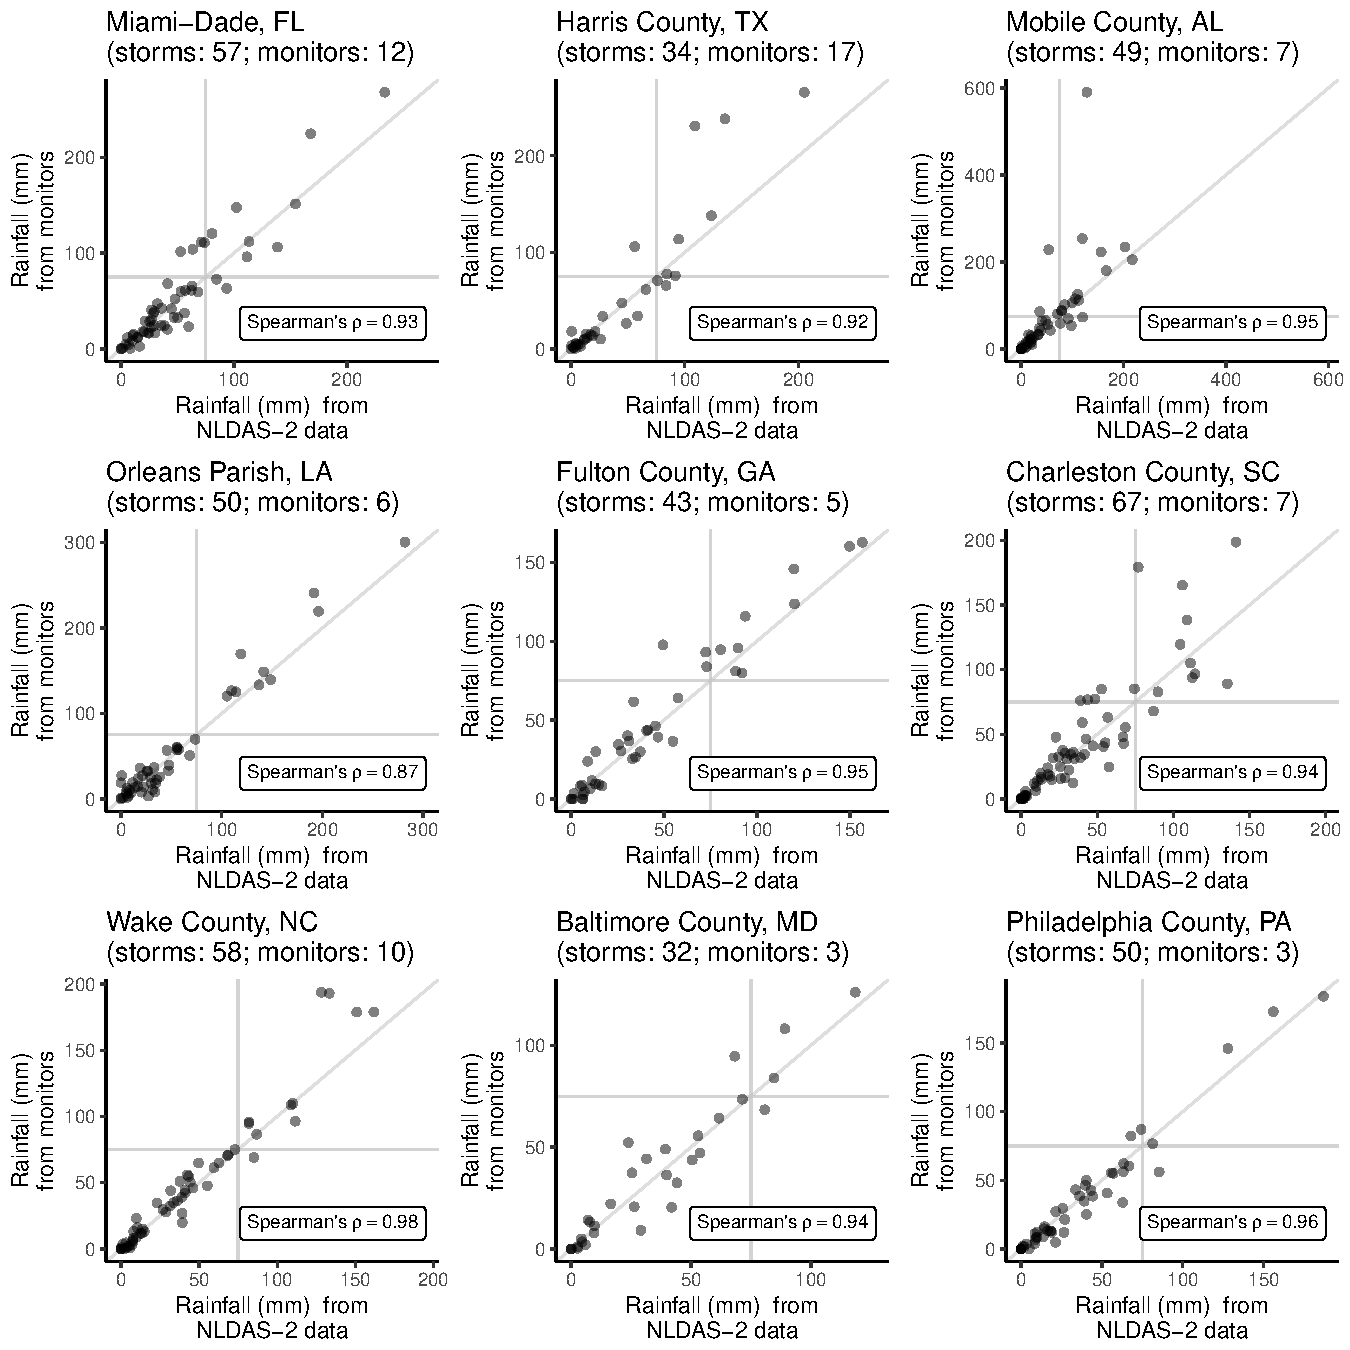
\includegraphics[width=0.9\linewidth]{raincomparison} 
	\caption{Comparison of storm-associated rainfall estimates between 
	a re-analysis dataset (included as the rainfall exposure metric
	in the open-source data and included in further analysis) and ground-based
	observations in nine sample counties. The rainfall estimates  
	include rainfall from two days before to one day after the storm's closest
	approach to the county. Each small graph shows data for one sample county, 
	and each point shows one tropical storm. The number of storms 
	within each county and the number of stations reporting rainfall during 
	the county's storms are given above each plot. Horizontal and vertical lines 
	in each plot show the threshold of 75~\si{\milli\metre} used to classify a storm 
	as ``exposed'' in further analysis (Table 1). Note that 
	ranges of the x and y axes differ across counties.
	} 
\label{fig:raincomparison}
\end{figure}

\begin{figure}[tbhp!]
\centering
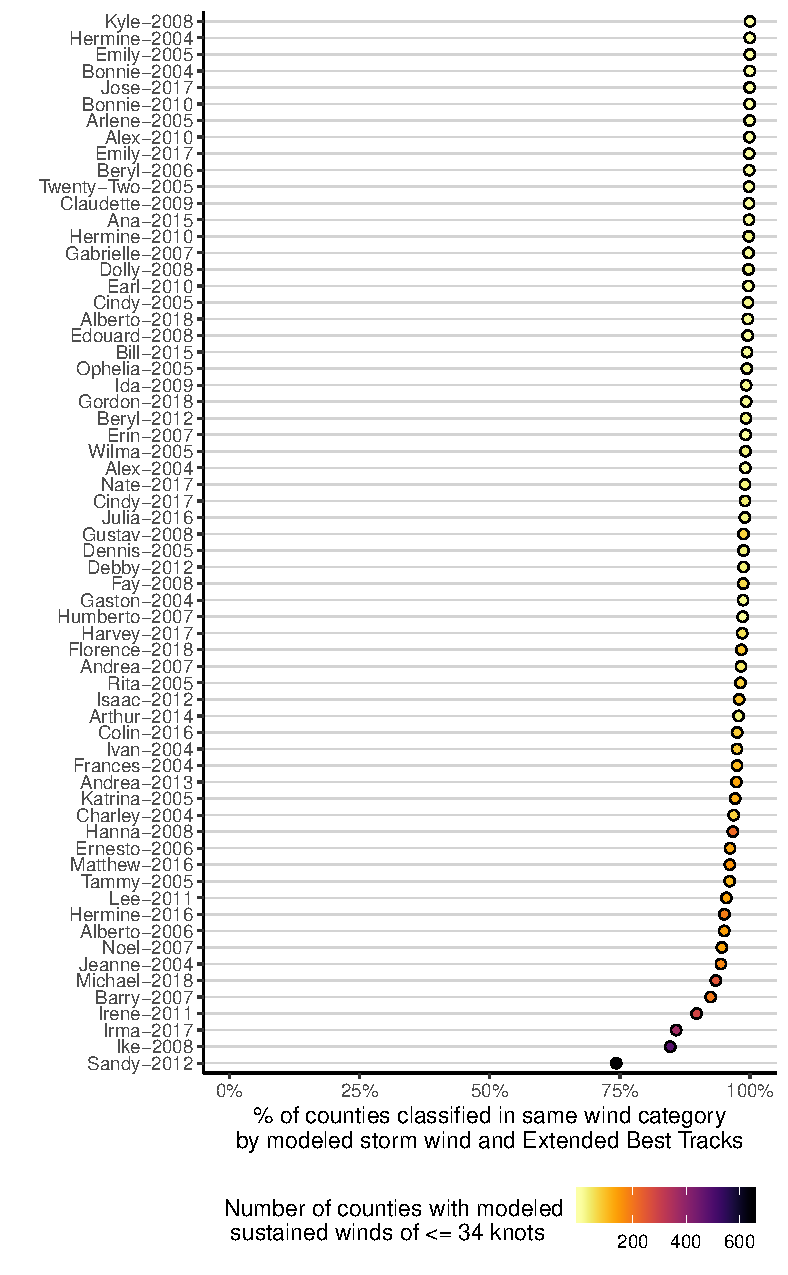
\includegraphics[width=0.6\linewidth]{windcomparison}
\caption{Comparison of modeled maximum sustained surface wind speeds (included
	as the primary wind exposure metric in the open-source data and used in
	further analysis) with estimates from \ac{HURDAT2}'s wind speed radii.
	Each point represents a storm, with the x axis giving the percent of
	counties classified in the same category of maximum sustained surface
	wind speeds ($<$34~\si{\knot}; 34\,--\,49.9~\si{\knot};
	50\,--\,63.9~\si{\knot}; $\ge$64~\si{\knot}) by both sources of wind
	data for that storm. The color of each point indicates the extent of
	the storm, giving the number of study counties that were exposed to
	maximum sustained surface wind speeds of at least 34~\si{\knot} (based
	on modeled wind speeds). Estimates are shown for study storms since
	2004, the earliest year for which post-storm reanalysis wind speed
	radii estimates are routinely available in \ac{HURDAT2}, for which at
	least one study county had a sustained wind speed of $\ge$34~\si{\knot}
	based on the \ac{HURDAT2} wind radii.
	}
\label{fig:windcomparison}
\end{figure}

\begin{figure}[tbhp!]
\centering
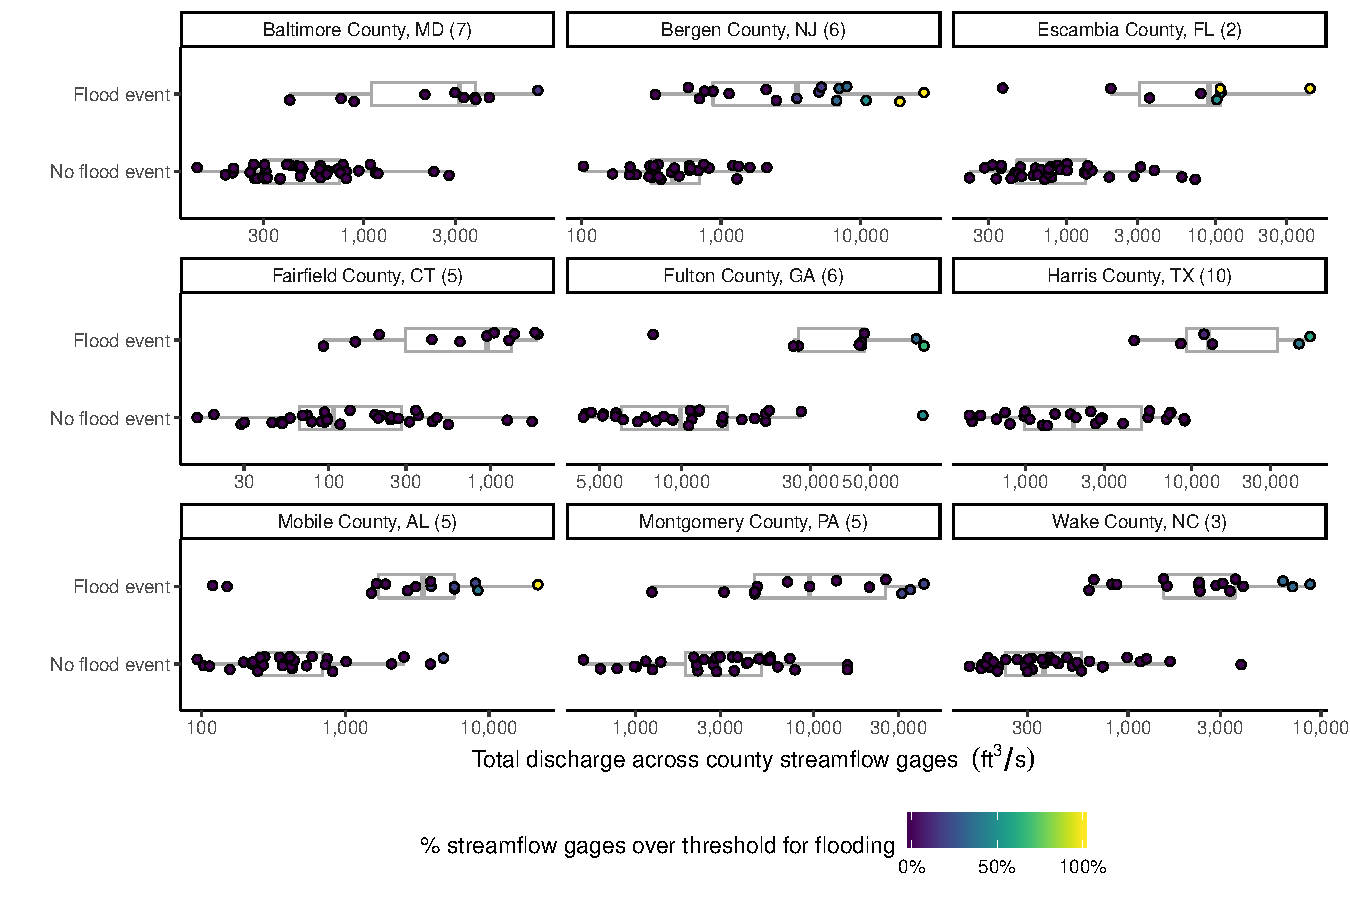
\includegraphics[width=0.8\linewidth]{floodcomparison}
\caption{Comparison for a sample of study counties of flood status based on
	matching NOAA Storm Events listings to \ac{HURDAT2} storm track data
	versus five-day total streamflows at county streamflow gages during
	tropical cyclones. Each small plot shows results for one of the sample
	counties. Each point represents a single tropical storm, and the
	point's position along the x-axis shows the highest daily total
	streamflow (cubic feet per second), summed across all identified
	streamgages in the county, for a five-day window centered on the day of
	the storm's closest approach to the county. The y-axis separates storms
	for which a flood event was reported in NOAA's Storm Events database
	for the county with a start date within the five-day window of the
	storm's closest approach to the county. The color of each point gives
	the percent of streamflow gages in the county with a daily streamflow
	that exceeded a threshold of flooding (the streamgage's median value
	for annual peak flow) on any day during the five-day window. The number
	of streamflow gages used in analysis are given in parentheses beside
	the county's name in the panel title.  Note that the x-axis scales
	differ by county, depending on the number of streamflow gages and
	typical flow rates for each gage, and are on a log-10 scale.
	}
\label{fig:floodcomparison}
\end{figure}

\clearpage

\begin{figure}%[tbhp] 
\centering
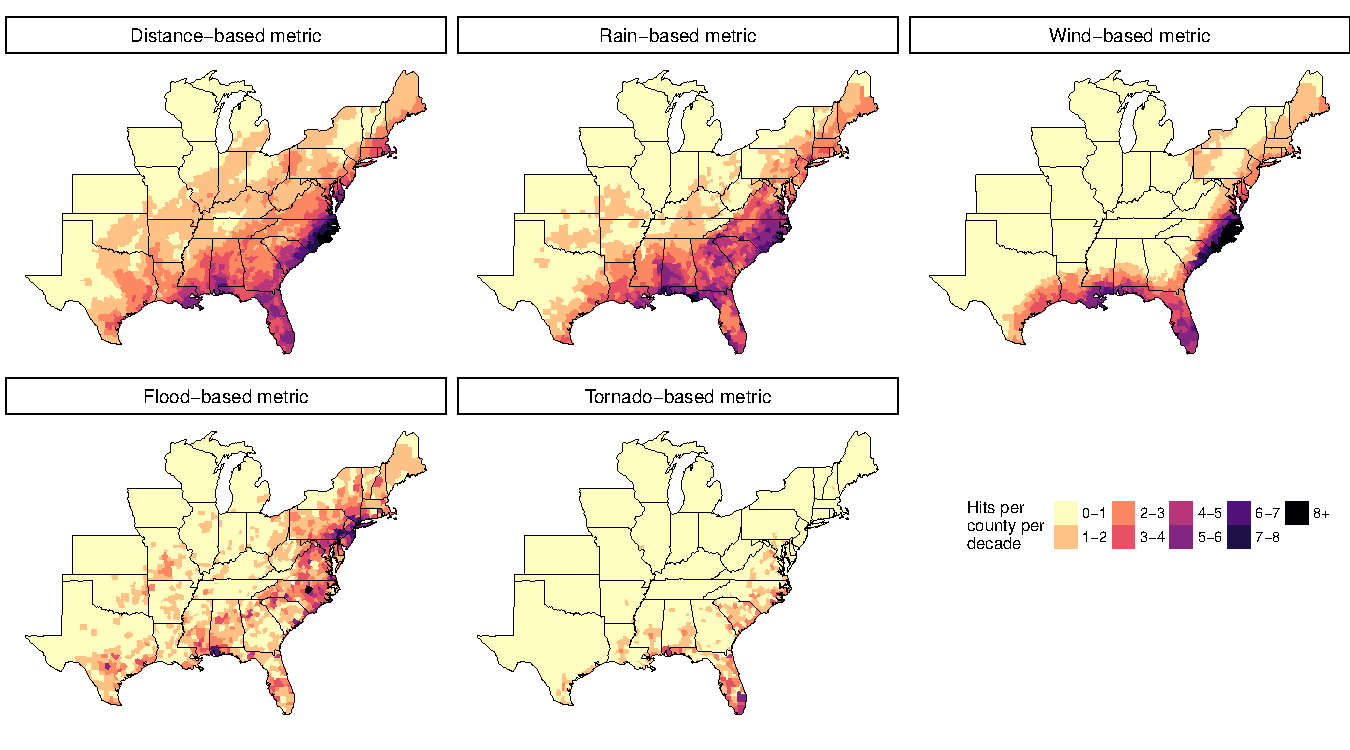
\includegraphics[width=7cm]{averageexposureonly.pdf} 
\caption{Average number of county-level storm exposures per decade for each
	single-hazard exposure metric. The criteria behind each of the five
	metrics is given in Table \ref{tab:exposuremetrics}. The years used to
	estimate these averages are based on years of available exposure data
	(rain: 1988\,--\,2011; wind:~1988\,--\,2015; flood and
	tornado events:~1996\,--\,2015). } 
\label{fig:averageexposure} 
\end{figure}

\clearpage

\begin{figure}%[tbhp]
\centering
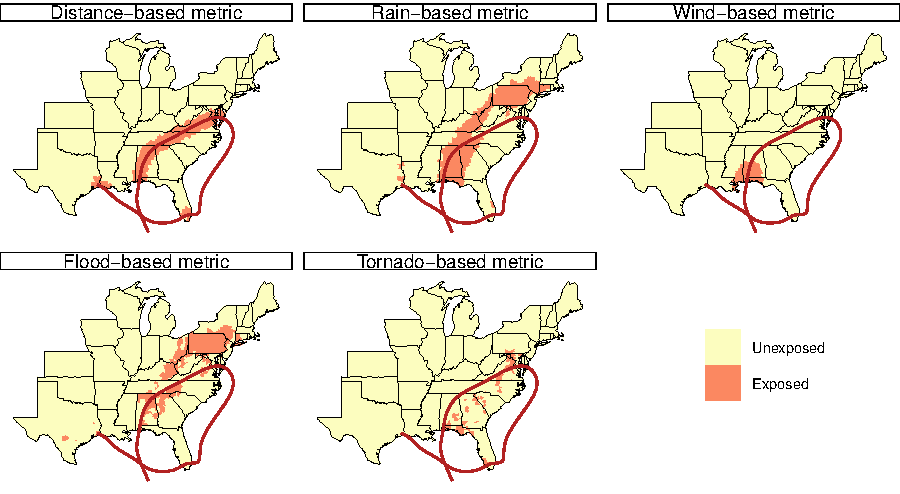
\includegraphics[width=16cm]{ivanonly.pdf}
\caption{Counties classified as exposed to Hurricane Ivan in 2004 under each
	exposure metric considered (Table~\ref{tab:exposuremetrics}). The red
	line shows the track of Hurricane Ivan based on
	\ac{HURDAT2}~\parencite{landsea2013}.  Similar maps for other
	large-extent storms are given in Figure~S4.
	}
\label{fig:ivanexposure} 
\end{figure}

\clearpage

\begin{figure}%[tbhp] 
\centering 
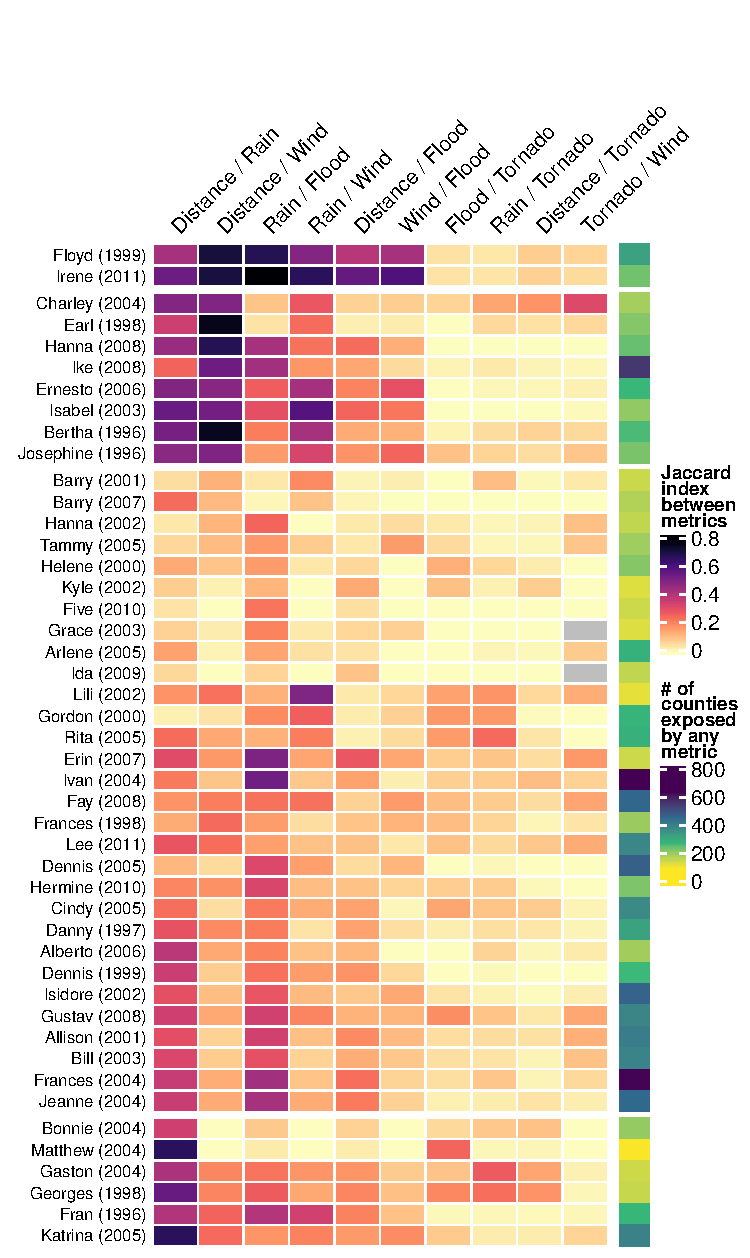
\includegraphics[width = 0.6\linewidth]{jaccard_heatmap.pdf} 
\caption{Agreement between exposure classifications based on different
         exposure metrics for all storms between~1996 and~2011 for which 
	 at least~250 counties were exposed based on at least one metric.
	 Each row shows one storm, and the color of each cell shows the 
	 measured Jaccard index for each pair of exposure metrics 
	 (proportion of counties classified as exposed by both metrics out 
	 of storms classified as exposed by either metric). The colors to the 
	 right of the main heatmap for each storm indicate the total number of 
	 counties classified as exposed to the storm by any of the five metrics, 
	 providing an indication of each storm's extent. Storms are displayed 
	 within clusters that have similar patterns in county-level exposure 
	 agreement for metric pairs, based on hierarchical clustering using the 
	 complete link method~\parencite{murtagh2012algorithms}; columns are also 
	 ordered based on hierarchical clustering. Maps are available showing the 
	 counties identified as exposed under each of five metrics for the widest-extent 
	 storm in each cluster: Hurricane Ivan in~2004 (Figure~\ref{fig:ivanexposure}) 
	 and Hurricanes Floyd in~1999, Lee in~2011, Cindy in~2005, and Katrina 
	 in~2005 (Figure~S4).
} 
\label{fig:jaccard}
\end{figure}

\clearpage

\begin{figure*}%[tbhp]
\centering
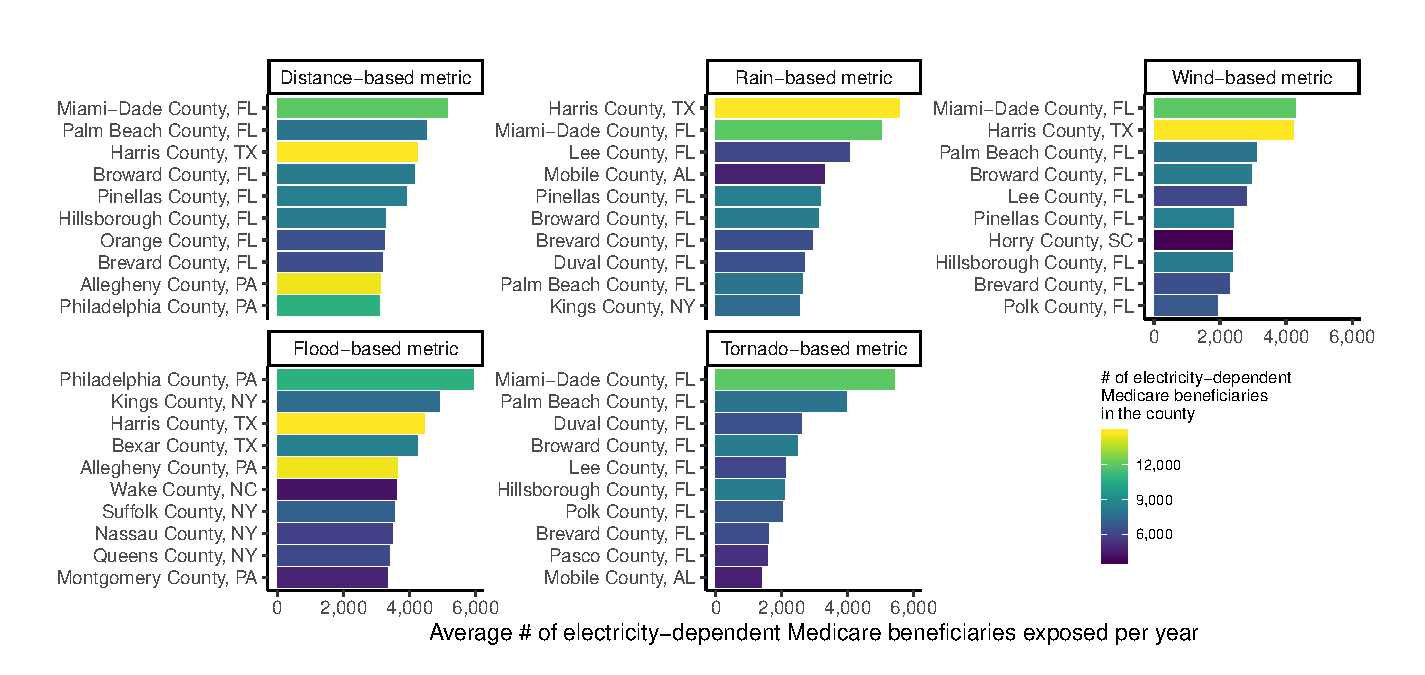
\includegraphics[width=15.5cm]{topelecdependexposure}
\caption{Study counties with the highest expected physical exposure per year among
	 electricity-dependent Medicare beneficiaries for each exposure metric. 
	 The color of each bar indicates the number of Medicare beneficiaries in the 
	 county reliant on electricity-dependent medical and assistive equipment as 
	 of July~2017. The length of each bar shows the average expected physical exposure
	 to tropical cyclones among this population based on a given exposure metric, i.e., 
	 the expected number of these electricity-dependent Medicare beneficiaries exposed 
	 to tropical storms per year based on that metric.}
\label{fig:topelecdependexposure}
\end{figure*}


